% catalogue: title = Layered network drawn with nested loops
% catalogue: min-coverage = 1.00
\documentclass[border=10pt]{standalone}
\PassOptionsToPackage{dvipsnames,svgnames,x11names}{xcolor}
\usepackage{tikz}
\usepackage{pgfplots}
\pgfplotsset{compat=newest}
\usepgfplotslibrary{groupplots}
\usetikzlibrary{arrows.meta}
\begin{document}
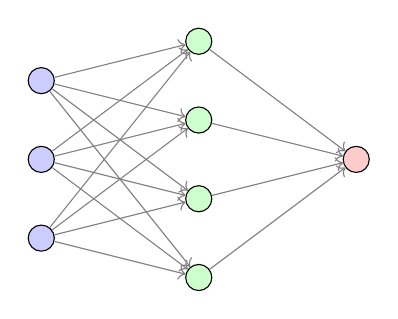
\begin{tikzpicture}
    \foreach \i in {1,2,3} {
        \node[circle, draw, fill=blue!20] (I\i) at (0, -\i) {};
    }
    \foreach \j in {1,2,3,4} {
        \node[circle, draw, fill=green!20] (H\j) at (2, {0.5 - \j}) {};
    }
    \node[circle, draw, fill=red!20] (O) at (4, -2) {};
    \foreach \i in {1,2,3} {
        \foreach \j in {1,2,3,4} {
            \draw[->, gray] (I\i) -- (H\j);
        }
    }
    \foreach \j in {1,2,3,4} {
        \draw[->, gray] (H\j) -- (O);
    }
\end{tikzpicture}
\end{document}
